% ====================================================================
% CAPÍTULO 3: ARQUITECTURA DE ChatHCE
% Trabajo Fin de Máster - AI Engineering
% Capítulo principal: visión de alto nivel, muy visual
% ====================================================================
% Paquetes requeridos en el preámbulo del documento maestro:
%   inputenc(utf8), fontenc(T1), babel(spanish), amsmath, amssymb,
%   graphicx, booktabs, longtable, array, tabularx, enumitem, float,
%   listings, xcolor, hyperref, tikz, pgfplots
%   \usetikzlibrary{shapes.geometric,shapes.multipart,arrows.meta,
%     positioning,calc,fit,backgrounds,decorations.pathreplacing}
%   \pgfplotsset{compat=1.18}
%   Requiere natbib o biblatex con comando \citep
% ====================================================================
%
% Paquetes adicionales necesarios en el preámbulo del documento principal:
%   \usepackage{amsthm}
%   \usepackage{thmtools}
%   \usepackage{tcolorbox}
%   \tcbuselibrary{skins,breakable}
%   \usepackage{listings}
%   \usetikzlibrary{shapes.geometric,arrows.meta,positioning,fit,
%                   backgrounds,calc,decorations.pathreplacing}
%
% Colores (escala de grises académica):
%   \definecolor{primary}{HTML}{2C3E50}
%   \definecolor{secondary}{HTML}{2980B9}
%   \definecolor{success}{HTML}{27AE60}
%   \definecolor{accent}{HTML}{E74C3C}
%   \definecolor{warning}{HTML}{F39C12}
%   \definecolor{codebg}{HTML}{F8F9FA}
%
% Entornos matemáticos:
%   \theoremstyle{definition}
%   \newtheorem{definition}{Definición}[section]
%   \newtheorem{proposition}{Proposición}[section]
% ====================================================================

\chapter{Arquitectura de ChatHCE}
\label{cap:arquitectura}

% ====================================================================
\section{Introducción y motivación clínica}
\label{sec:introduccion}
% ====================================================================

El ejercicio de la medicina de urgencias impone una carga cognitiva y temporal excepcional sobre los profesionales sanitarios. Un médico de urgencias necesita acceder, de forma simultánea y en tiempo real, a tres categorías de información heterogéneas: datos estructurados del paciente almacenados en bases de datos relacionales (signos vitales, diagnósticos previos, medicación activa), conocimiento clínico no estructurado contenido en guías y protocolos (documentos PDF, DOCX), y representaciones visuales que permitan identificar tendencias en series temporales de parámetros fisiológicos. Esta integración se realiza habitualmente mediante múltiples sistemas desconectados, con interfaces distintas y sin capacidad de consulta en lenguaje natural. Recientes revisiones sistemáticas han documentado el potencial de los modelos de lenguaje de gran escala para tareas clínicas como resumen, consulta de conocimiento y predicción \parencite{wang2024chatgpt}.

Según \textcite{arun2025ethical}, los médicos dedican una media de 16 minutos y 14 segundos de tiempo activo en el sistema de historia clínica electrónica (\acs{HCE}) por cada encuentro con el paciente, lo que representa entre el 37\% y el 49\% del tiempo total de la visita. En urgencias, donde los tiempos de respuesta son críticos, esta carga documental puede comprometer la calidad asistencial. El sistema \textbf{AgentClinic} \parencite{AgentClinic2025} ha demostrado que los agentes conversacionales pueden simular entornos clínicos completos, mientras que revisiones como las de \textcite{Amugongo2025systematic} confirman la viabilidad de sistemas \ac{RAG} en el dominio sanitario.

\textbf{ChatHCE} aborda este problema proporcionando una interfaz conversacional unificada en lenguaje natural que integra automáticamente las tres fuentes de información mediante selección inteligente de herramientas. El sistema opera sobre el dataset \acs{MIMIC}-IV-\acs{ED} \parencite{johnson2023mimiciv}, un conjunto de datos clínicos anonimizados ampliamente utilizado en investigación biomédica, y ha sido diseñado para responder a cinco preguntas de investigación fundamentales que guían su arquitectura técnica.

\subsection{Preguntas de investigación}

Este capítulo describe la arquitectura de ChatHCE en función de cinco preguntas de investigación (\acs{RQ}) que abordan los principales desafíos técnicos de un sistema conversacional clínico:

\begin{description}[nosep, leftmargin=1em, labelindent=0em]
  \item[\textbf{RQ1}:] ¿Cómo puede una \textbf{arquitectura de agente unificado} con \textit{tool-calling} nativo alcanzar latencias P50 inferiores a 5 segundos mientras reduce el error acumulado en comparación con arquitecturas multi-agente?
  
  \item[\textbf{RQ2}:] ¿En qué medida la \textbf{búsqueda híbrida} (vectorial + léxica) combinada con \textit{Reciprocal Rank Fusion} (\ac{RRF}, $k=60$) y \textbf{chunking jerárquico} padre-hijo mejora la precisión de recuperación respecto a búsqueda vectorial pura?
  
  \item[\textbf{RQ3}:] ¿Cómo implementar una estrategia de \textbf{defensa en profundidad} con múltiples capas de seguridad (validación \ac{SQL}, sandbox \ac{AST}, directivas de prompt) para mitigar alucinaciones y garantizar la integridad de los datos clínicos?
  
  \item[\textbf{RQ4}:] ¿Qué mecanismos de \textbf{fallback} (Haiku $\rightarrow$ Sonnet $\rightarrow$ Opus) garantizan la continuidad operativa ante fallos de \ac{API} o rate limiting?
  
  \item[\textbf{RQ5}:] ¿Cuáles son los beneficios de un enfoque \textbf{\textit{template-first}} en visualización ($\sim$0.4\,s) frente a generación por \ac{LLM} ($\sim$4\,s) en términos de latencia y determinismo?
\end{description}

Las siguientes secciones describen cómo la arquitectura de ChatHCE responde a cada una de estas preguntas. Para un análisis técnico exhaustivo de cada componente, véase el Anexo~\ref{appendix:arquitectura}.

% ====================================================================
\section{Visión general del sistema}
\label{sec:vision}
% ====================================================================

\subsection{Descripción funcional}

\textbf{ChatHCE} es un sistema de análisis clínico inteligente diseñado para profesionales del Servicio de Urgencias que necesitan acceder, en tiempo real y mediante lenguaje natural en español, a datos de pacientes del dataset \acs{MIMIC}-IV-\acs{ED}, guías clínicas indexadas y visualizaciones interactivas. El sistema opera como una interfaz conversacional única que elimina la necesidad de cambiar entre múltiples aplicaciones o aprender lenguajes de consulta especializados.

El sistema se articula sobre tres pilares tecnológicos complementarios:

\begin{enumerate}[nosep, leftmargin=*]
  \item Un \textbf{agente conversacional unificado} basado en Claude Haiku 4.5 con capacidad de \textit{tool\mbox{-}calling} nativo, que analiza la intención del usuario y selecciona automáticamente las herramientas apropiadas (\textbf{RQ1}).
  \item Un \textbf{pipeline RAG} (\textit{Retrieval-Augmented Generation}) con búsqueda híbrida vectorial-léxica, fusión \ac{RRF} y chunking jerárquico sobre Supabase~\parencite{supabase2020} pgvector~\parencite{pgvector2024}, que recupera fragmentos relevantes de documentos clínicos indexados (\textbf{RQ2}).
  \item Un \textbf{motor de visualización} con enfoque \textit{template\mbox{-}first} que genera gráficas interactivas con Plotly~\parencite{plotly2015} a partir de datos clínicos, activándose automáticamente cuando la consulta implica tendencias temporales (\textbf{RQ5}).
\end{enumerate}

\subsection{Formalización matemática}
\label{sec:formalizacion}

Se formaliza el problema de análisis clínico conversacional de la siguiente manera. El dataset clínico se define como $\mathcal{D} = \{T_1, T_2, \ldots, T_6\}$, donde cada $T_i$ es una tabla relacional del esquema \texttt{mimic\_ed}. La base de conocimiento documental se define como $\mathcal{K} = \{c_1, c_2, \ldots, c_n\}$, donde cada $c_i$ es un fragmento de texto clínico con embedding asociado $\mathbf{e}_i \in \mathbb{R}^{384}$.

El sistema ChatHCE se modela como una función de síntesis:

\begin{equation}
f: \mathcal{Q} \times \mathcal{D} \times \mathcal{K} \rightarrow \mathcal{R}
\label{eq:sistema}
\end{equation}

donde $\mathcal{Q}$ es el espacio de consultas en lenguaje natural y $\mathcal{R}$ son tuplas $(r_\text{texto}, V_\text{viz}, S_\text{fuentes})$. La función $f$ se descompone mediante selección dinámica de herramientas:

\begin{equation}
f(q, \mathcal{D}, \mathcal{K}) = \mathcal{A}\!\left(\,f_\text{DB}(q,\,\mathcal{D}),\; f_\text{RAG}(q,\,\mathcal{K}),\; f_\text{VIZ}(q,\,\mathcal{D})\,\right)
\label{eq:descomposicion}
\end{equation}

donde $\mathcal{A}$ es la función de síntesis del agente y el subconjunto de herramientas a invocar se determina dinámicamente: $\mathcal{T}(q) \subseteq \{\text{DB},\, \text{RAG},\, \text{VIZ}\}$.

\subsection{Flujo de procesamiento de alto nivel}

El procesamiento de una consulta sigue ocho etapas secuenciales (Figura~\ref{fig:flujo_end2end}): recepción de la consulta en Streamlit, verificación de caché (\ac{TTL}: 300\,s), análisis de intención por Claude Haiku 4.5, selección dinámica de herramientas ($\mathcal{T}(q)$), ejecución de las herramientas seleccionadas (hasta 5 iteraciones), y síntesis final de la respuesta integrada.

\begin{figure*}[t]
\centering
\resizebox{\textwidth}{!}{%
\begin{tikzpicture}[
  ionode/.style={
    draw=black!70, fill=gray!8, rounded corners=4pt,
    minimum width=4.5cm, minimum height=0.8cm,
    font=\small\sffamily\bfseries, align=center
  },
  procnode/.style={
    draw=black!60, fill=gray!5, rounded corners=3pt,
    minimum width=4.5cm, minimum height=0.75cm,
    font=\small\sffamily, align=center
  },
  toolnode/.style={
    draw=black!60, fill=gray!10, rounded corners=3pt,
    minimum width=3.2cm, minimum height=0.7cm,
    font=\small\sffamily\bfseries, align=center
  },
  decnode/.style={
    draw=black!60, fill=gray!8, diamond, aspect=2.8,
    font=\small\sffamily, align=center,
    inner sep=2pt
  },
  flowarrow/.style={
    -{Stealth[length=6pt]}, thick, color=black!60
  },
  latency/.style={
    font=\tiny\sffamily\itshape, text=gray!60, anchor=west
  }
]

\node[ionode] (user)    at (0, 0)    {Usuario escribe consulta en español};
\node[procnode] (cache)  at (0,-1.5)  {Verificación de caché (\ac{TTL}: 300\,s)};
\node[procnode] (claude) at (0,-3.0)  {Claude Haiku 4.5 analiza intención};
\node[decnode] (select) at (0,-4.6) {$\mathcal{T}(q)$: selección de herramientas};

\node[toolnode]  (db)  at (-4.5,-6.5) {Database Tool\\$f_\text{DB}$};
\node[toolnode]  (rag) at ( 0.0,-6.5) {RAG Tool\\$f_\text{RAG}$};
\node[toolnode]  (viz) at ( 4.5,-6.5) {Visualization Tool\\$f_\text{VIZ}$};

\node[procnode, minimum width=5.5cm] (synth) at (0,-8.5) {Claude sintetiza respuesta integrada $\mathcal{A}(\cdot)$};
\node[ionode]   (out)   at (0,-10.0) {Respuesta + Gráficas interactivas + Fuentes};

\draw[flowarrow] (user)   -- (cache);
\draw[flowarrow] (cache)  -- (claude);
\draw[flowarrow] (claude) -- (select);

\coordinate (junc) at (0,-5.4);
\draw[flowarrow] (select.south) -- (junc);
\draw[flowarrow] (junc) -- (rag.north);
\draw[flowarrow] (junc) -| (db.north);
\draw[flowarrow] (junc) -| (viz.north);

\draw[flowarrow] (db.south)  |- (synth.west);
\draw[flowarrow] (rag.south) -- (synth.north);
\draw[flowarrow] (viz.south) |- (synth.east);

\draw[flowarrow] (synth) -- (out);

\node[latency] at (7.5, -1.5)  {$\sim$5\,ms (hit)};
\node[latency] at (7.5, -3.0)  {P50: $\sim$800\,ms};
\node[latency] at (7.5, -6.5)  {P50: $\sim$1.5\,s / $\sim$2\,s / $\sim$3\,s};
\node[latency] at (7.5, -8.5)  {P50: $\sim$1\,s};
\node[latency] at (7.5, -10.0) {Total P50: $<$5\,s};

\end{tikzpicture}%
}% end resizebox
\caption{Flujo \textit{end-to-end} de una consulta en ChatHCE. Las anotaciones laterales indican latencias objetivo (P50). El agente selecciona dinámicamente el subconjunto $\mathcal{T}(q)$ de herramientas a invocar. El objetivo de latencia P50 $<$ 5\,s responde a \textbf{RQ1}.}
\label{fig:flujo_end2end}
\end{figure*}

% ====================================================================
\section{Arquitectura de agente unificado (\acs{RQ}1)}
\label{sec:agente_unificado}
% ====================================================================

La decisión arquitectónica más relevante del sistema es la adopción de un \textbf{agente unificado} (\texttt{UnifiedChatAgent}) en lugar de una arquitectura multi-agente. Esta decisión responde a tres requisitos críticos del dominio clínico: (1)~latencia mínima, dado que una arquitectura multi-agente requiere 3--5 llamadas \ac{LLM} secuenciales multiplicando la latencia; (2)~reducción del error acumulado, ya que el agente unificado sintetiza directamente desde los resultados sin transformaciones intermedias; y (3)~\textit{tool-calling} determinista, donde Claude Haiku 4.5 genera estructuras \ac{JSON} nativas especificando herramienta y parámetros, eliminando el parsing de texto libre propenso a errores \parencite{Wang2024SurveyAgents}.

\subsection{Comparativa con arquitectura multi-agente}

La Figura~\ref{fig:comparativa_agentes} ilustra la diferencia estructural entre ambos enfoques. La arquitectura multi-agente requiere múltiples nodos de procesamiento \ac{LLM} coordinados, mientras que el agente unificado centraliza la orquestación en un único nodo con acceso directo a herramientas.

\begin{figure*}[t]
\centering
\resizebox{\textwidth}{!}{%
\begin{tikzpicture}[
  agentnode/.style={
    draw=black!55, fill=gray!8, rounded corners=3pt,
    minimum height=0.7cm,
    font=\small\sffamily, align=center
  },
  toolnode/.style={
    draw=black!55, fill=gray!15, rounded corners=3pt,
    minimum height=0.6cm,
    font=\small\sffamily\bfseries, align=center
  },
  disadvlabel/.style={
    font=\tiny\sffamily\itshape, text=black!60, align=left
  },
  advlabel/.style={
    font=\tiny\sffamily\itshape, text=black!70, align=left
  },
  flowarrow/.style={
    -{Stealth[length=5pt]}, thick, color=black!50
  }
]

% COLUMNA IZQUIERDA: Multi-Agente (descartado)
\node[font=\small\sffamily\bfseries, text=black!60] at (-6.0, 4.5) {Arquitectura Multi-Agente};
\node[font=\tiny\sffamily\itshape, text=gray!60] at (-6.0, 4.1) {(alternativa descartada)};

\node[agentnode, minimum width=3.0cm] (orch) at (-6.0, 3.2) {OrchestratorAgent};
\node[agentnode, minimum width=2.0cm] (dba)  at (-8.5, 1.8) {DBAgent};
\node[agentnode, minimum width=2.0cm] (raga) at (-6.0, 1.8) {RAGAgent};
\node[agentnode, minimum width=2.0cm] (viza) at (-3.5, 1.8) {VizAgent};
\node[agentnode, minimum width=3.0cm] (critic) at (-6.0, 0.4) {CriticAgent};
\node[agentnode, minimum width=3.0cm] (resp1) at (-6.0, -0.8) {Respuesta};

\draw[flowarrow] (orch) -- (dba);
\draw[flowarrow] (orch) -- (raga);
\draw[flowarrow] (orch) -- (viza);
\draw[flowarrow] (dba) |- (critic);
\draw[flowarrow] (raga) -- (critic);
\draw[flowarrow] (viza) |- (critic);
\draw[flowarrow] (critic) -- (resp1);

\node[disadvlabel, anchor=north] at (-6.0, -1.5) {%
  $\times$ 3--5 llamadas \ac{LLM} por turno\\
  $\times$ Error acumulado entre nodos\\
  $\times$ Latencia $>$ 10\,s (estimada)};

% SEPARADOR CENTRAL
\draw[very thick, gray!30, dashed] (0, -2.5) -- (0, 5.0);
\node[font=\large\sffamily\bfseries, text=gray!50] at (0, 1.2) {vs.};

% COLUMNA DERECHA: Agente Unificado (adoptado)
\node[font=\small\sffamily\bfseries, text=black!70] at (6.0, 4.5) {Agente Unificado ChatHCE};
\node[font=\tiny\sffamily\itshape, text=gray!60] at (6.0, 4.1) {(decisión adoptada)};

\node[agentnode, minimum width=3.8cm, draw=black!70] (unified) at (6.0, 3.2) {UnifiedChatAgent\\Claude Haiku 4.5};

\node[toolnode, minimum width=2.0cm] (dbt)  at (3.5, 1.8) {DB Tool};
\node[toolnode, minimum width=2.0cm] (ragt) at (6.0, 1.8) {RAG Tool};
\node[toolnode, minimum width=2.0cm] (vizt) at (8.5, 1.8) {VIZ Tool};

\node[agentnode, minimum width=3.8cm] (synth2) at (6.0, 0.4) {Síntesis directa\\(una sola llamada \ac{LLM})};
\node[agentnode, minimum width=3.8cm] (resp2) at (6.0, -0.8) {Respuesta integrada};

\draw[flowarrow] (unified) -- (dbt);
\draw[flowarrow] (unified) -- (ragt);
\draw[flowarrow] (unified) -- (vizt);
\draw[flowarrow] (dbt) |- (synth2);
\draw[flowarrow] (ragt) -- (synth2);
\draw[flowarrow] (vizt) |- (synth2);
\draw[flowarrow] (synth2) -- (resp2);

\node[advlabel, anchor=north] at (6.0, -1.5) {%
  $\checkmark$ 1 llamada \ac{LLM} por turno\\
  $\checkmark$ Síntesis directa sin intermediarios\\
  $\checkmark$ Latencia P50 $<$ 5\,s};

% Caja de fallback
\node[agentnode, minimum width=2.8cm, draw=black!50, fill=gray!5] (fallback) at (11.5, 3.2) {Cadena fallback:\\Haiku $\rightarrow$ Sonnet $\rightarrow$ Opus};
\draw[flowarrow, dashed] (unified) -- (fallback);

\end{tikzpicture}%
}% end resizebox
\caption{Comparativa entre arquitectura multi-agente (izquierda, descartada) y agente unificado (derecha, adoptada). El agente unificado reduce llamadas \acs{LLM} de 3--5 a 1 por turno, eliminando error acumulado y reduciendo latencia. La cadena de fallback garantiza continuidad operativa (\textbf{RQ4}).}
\label{fig:comparativa_agentes}
\end{figure*}

\subsection{Componentes del agente unificado}

El \texttt{UnifiedChatAgent} se implementa como un \texttt{AgentExecutor} de LangChain con los siguientes componentes principales:

\begin{itemize}[nosep, leftmargin=*]
  \item \textbf{Motor LLM}: \texttt{ClaudeLLMManager} gestiona la comunicación con la \ac{API} de Anthropic. Claude Haiku 4.5 (\texttt{claude-haiku-4-5-20251001}) genera estructuras \ac{JSON} nativas para \textit{tool-calling}, eliminando parsing de texto libre.
  \item \textbf{Registro de herramientas}: \texttt{ClaudeToolRegistry} centraliza las tres herramientas mediante el patrón \textit{Adapter} (\texttt{ClaudeToolAdapter}).
  \item \textbf{Gestor de prompts}: \texttt{PromptManager} genera el prompt del sistema con límite de 8000 tokens, estructurado en 10 secciones (identidad, contexto, herramientas, anti-alucinación, idioma, esquema BD, herramientas detalladas, formato, guías clínicas, selección de herramientas).
\end{itemize}

La Tabla~\ref{tab:metricas_agente} resume las métricas objetivo del agente unificado.

\begin{table}[H]
\centering
\caption{Métricas de rendimiento del agente unificado (\textbf{RQ1}).}
\label{tab:metricas_agente}
\footnotesize
\begin{tabularx}{\columnwidth}{lXr}
\toprule
\textbf{Métrica} & \textbf{Descripción} & \textbf{Objetivo} \\
\midrule
Latencia P50 & Tiempo total extremo a extremo & $<$ 5\,s \\
Latencia P95 & Tiempo en percentil 95 & $<$ 8\,s \\
Llamadas \ac{LLM}/turno & Invocaciones al modelo por turno & 1 \\
Error acumulado & Errores por encadenamiento de agentes & 0 \\
Tasa de éxito tool-calling & Invocaciones correctas de herramientas & $>$ 95\% \\
\bottomrule
\end{tabularx}
\end{table}

Para una descripción detallada de la configuración del \texttt{AgentExecutor}, la interfaz \texttt{ClaudeToolAdapter} y el sistema de prompts de 10 secciones, véase el Anexo~\ref{appendix:arquitectura}.

% ====================================================================
\section{Arquitectura por capas del sistema}
\label{sec:arquitectura_capas}
% ====================================================================

ChatHCE sigue una arquitectura de cinco capas con separación estricta de responsabilidades, inspirada en el patrón \textit{Layered Architecture} \parencite{Fowler2002}. El principio rector es que cada capa solo puede comunicarse con la capa inmediatamente inferior. La Figura~\ref{fig:capas_interfaces} presenta la arquitectura completa con interfaces entre capas.

\begin{figure*}[t]
\centering
\resizebox{0.95\textwidth}{!}{%
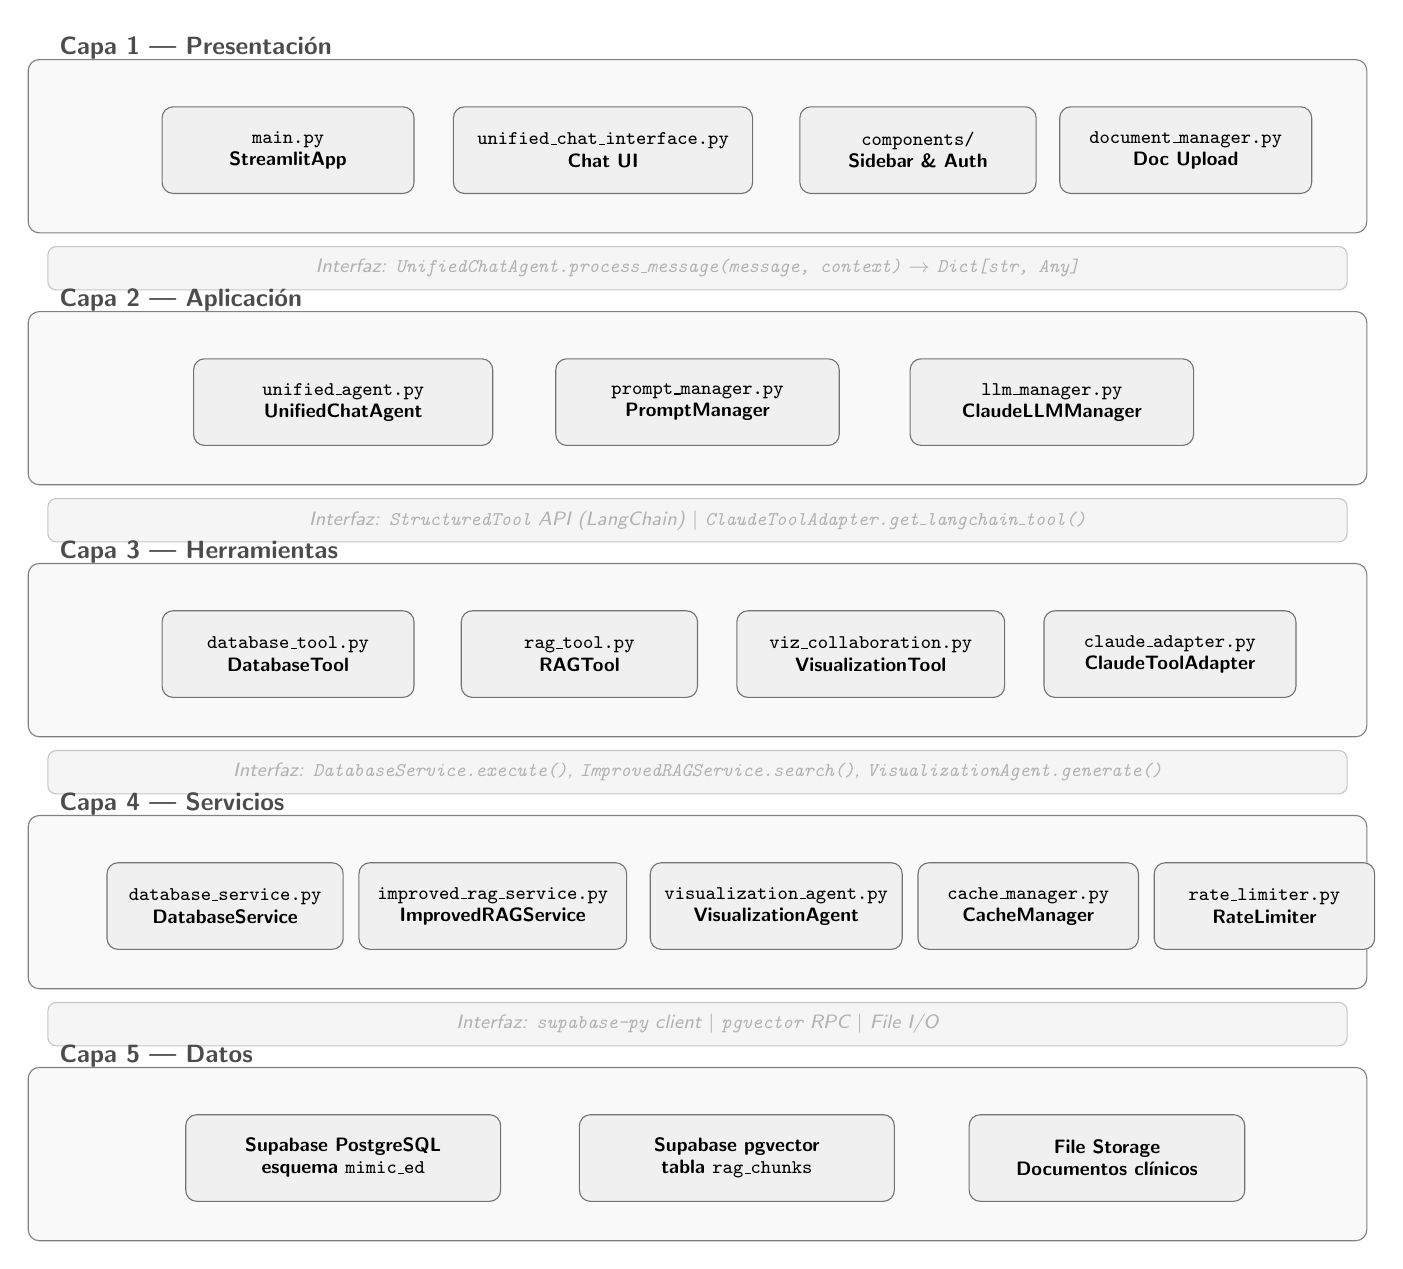
\begin{tikzpicture}[
  layerbox/.style={
    draw=black!50, fill=gray!5, rounded corners=4pt,
    minimum width=17cm, minimum height=2.2cm, inner sep=10pt,
    font=\small\sffamily
  },
  compbox/.style={
    draw=black!55, fill=gray!12, rounded corners=4pt,
    minimum height=1.1cm, font=\scriptsize\sffamily\bfseries,
    align=center, inner sep=5pt
  },
  ifacebox/.style={
    draw=gray!45, fill=gray!8, rounded corners=3pt,
    minimum height=0.55cm, font=\scriptsize\sffamily\itshape,
    text=gray!60, align=center, inner sep=4pt
  },
  layerlabel/.style={
    font=\small\sffamily\bfseries, text=black!70
  }
]

% Capa 1: Presentación
\node[layerbox] (L1) at (0, 0) {};
\node[layerlabel, anchor=west] at ([xshift=8pt, yshift=4pt]L1.north west) {Capa 1 --- Presentación};
\node[compbox, minimum width=3.2cm] at (-5.2, -0.05) {\texttt{main.py}\\StreamlitApp};
\node[compbox, minimum width=3.8cm] at (-1.2, -0.05) {\texttt{unified\_chat\_interface.py}\\Chat UI};
\node[compbox, minimum width=3.0cm] at (2.8, -0.05) {\texttt{components/}\\Sidebar \& Auth};
\node[compbox, minimum width=3.2cm] at (6.2, -0.05) {\texttt{document\_manager.py}\\Doc Upload};

% Interfaz 1-2
\node[ifacebox, minimum width=16.5cm] (I12) at (0, -1.55) {Interfaz: \texttt{UnifiedChatAgent.process\_message(message, context)} $\rightarrow$ \texttt{Dict[str, Any]}};

% Capa 2: Aplicación
\node[layerbox] (L2) at (0, -3.2) {};
\node[layerlabel, anchor=west] at ([xshift=8pt, yshift=4pt]L2.north west) {Capa 2 --- Aplicación};
\node[compbox, minimum width=3.8cm] at (-4.5, -3.25) {\texttt{unified\_agent.py}\\UnifiedChatAgent};
\node[compbox, minimum width=3.6cm] at (0.0, -3.25) {\texttt{prompt\_manager.py}\\PromptManager};
\node[compbox, minimum width=3.6cm] at (4.5, -3.25) {\texttt{llm\_manager.py}\\ClaudeLLMManager};

% Interfaz 2-3
\node[ifacebox, minimum width=16.5cm] (I23) at (0, -4.75) {Interfaz: \texttt{StructuredTool} \ac{API} (LangChain) $\mid$ \texttt{ClaudeToolAdapter.get\_langchain\_tool()}};

% Capa 3: Herramientas
\node[layerbox] (L3) at (0, -6.4) {};
\node[layerlabel, anchor=west] at ([xshift=8pt, yshift=4pt]L3.north west) {Capa 3 --- Herramientas};
\node[compbox, minimum width=3.2cm] at (-5.2, -6.45) {\texttt{database\_tool.py}\\DatabaseTool};
\node[compbox, minimum width=3.0cm] at (-1.5, -6.45) {\texttt{rag\_tool.py}\\RAGTool};
\node[compbox, minimum width=3.4cm] at (2.2, -6.45) {\texttt{viz\_collaboration.py}\\VisualizationTool};
\node[compbox, minimum width=3.2cm] at (6.0, -6.45) {\texttt{claude\_adapter.py}\\ClaudeToolAdapter};

% Interfaz 3-4
\node[ifacebox, minimum width=16.5cm] (I34) at (0, -7.95) {Interfaz: \texttt{DatabaseService.execute()}, \texttt{ImprovedRAGService.search()}, \texttt{VisualizationAgent.generate()}};

% Capa 4: Servicios
\node[layerbox] (L4) at (0, -9.6) {};
\node[layerlabel, anchor=west] at ([xshift=8pt, yshift=4pt]L4.north west) {Capa 4 --- Servicios};
\node[compbox, minimum width=3.0cm] at (-6.0, -9.65) {\texttt{database\_service.py}\\DatabaseService};
\node[compbox, minimum width=3.4cm] at (-2.6, -9.65) {\texttt{improved\_rag\_service.py}\\ImprovedRAGService};
\node[compbox, minimum width=3.2cm] at (1.0, -9.65) {\texttt{visualization\_agent.py}\\VisualizationAgent};
\node[compbox, minimum width=2.8cm] at (4.2, -9.65) {\texttt{cache\_manager.py}\\CacheManager};
\node[compbox, minimum width=2.8cm] at (7.2, -9.65) {\texttt{rate\_limiter.py}\\RateLimiter};

% Interfaz 4-5
\node[ifacebox, minimum width=16.5cm] (I45) at (0, -11.15) {Interfaz: \texttt{supabase-py} client $\mid$ \texttt{pgvector} RPC $\mid$ File I/O};

% Capa 5: Datos
\node[layerbox] (L5) at (0, -12.8) {};
\node[layerlabel, anchor=west] at ([xshift=8pt, yshift=4pt]L5.north west) {Capa 5 --- Datos};
\node[compbox, minimum width=4.0cm] at (-4.5, -12.85) {Supabase PostgreSQL\\esquema \texttt{mimic\_ed}};
\node[compbox, minimum width=4.0cm] at (0.5, -12.85) {Supabase pgvector\\tabla \texttt{rag\_chunks}};
\node[compbox, minimum width=3.5cm] at (5.2, -12.85) {File Storage\\Documentos clínicos};

\end{tikzpicture}%
}% end resizebox
\caption{Arquitectura por capas de ChatHCE con interfaces entre capas. Cada capa solo puede comunicarse con la capa inmediatamente inferior. Patrones de diseño: Adapter (\texttt{ClaudeToolAdapter}), Singleton (\texttt{CacheManager}, \texttt{RateLimiter}, \texttt{ImprovedRAGService}), Strategy (búsqueda \acs{RAG}), Factory (\texttt{ClaudeToolRegistry}), Chain of Responsibility (fallback \acs{LLM}).}
\label{fig:capas_interfaces}
\end{figure*}

\textbf{Capa 1 --- Presentación.} Implementada con Streamlit, gestiona la interfaz de usuario, el chat interactivo, la autenticación y la carga de documentos para el sistema \ac{RAG}. No contiene lógica de negocio.

\textbf{Capa 2 --- Aplicación.} Contiene la lógica de orquestación: \texttt{UnifiedChatAgent} recibe la consulta, gestiona el historial conversacional, invoca herramientas y sintetiza la respuesta. \texttt{PromptManager} genera el prompt del sistema (8000 tokens máximo, 10 secciones) y \texttt{ClaudeLLMManager} gestiona la cadena de fallback entre modelos.

\textbf{Capa 3 --- Herramientas.} Tres herramientas especializadas adaptadas a LangChain mediante el patrón \textit{Adapter}: \texttt{DatabaseTool} (consultas \ac{SQL} validadas), \texttt{RAGTool} (búsqueda híbrida en documentos) y \texttt{VisualizationTool} (gráficas Plotly).

\textbf{Capa 4 --- Servicios.} Servicios de infraestructura: \texttt{DatabaseService}, \texttt{ImprovedRAGService} (pipeline \ac{RAG} completo), \texttt{VisualizationAgent}, \texttt{CacheManager} (\ac{LRU} con \ac{TTL}=300s) y \texttt{RateLimiter} (30 req/min, 300 req/hora).

\textbf{Capa 5 --- Datos.} Backend unificado en Supabase: PostgreSQL 15 con esquema \texttt{mimic\_ed}, pgvector 0.8.0 con tabla \texttt{rag\_chunks}, y almacenamiento de archivos para documentos clínicos originales.

Para una descripción completa de las tablas, índices y esquemas de datos, véase el Anexo~\ref{appendix:arquitectura}.

% ====================================================================
\section{Fuente de datos: \acs{MIMIC}-IV-ED}
\label{sec:mimic}
% ====================================================================

Como se describió en la Sección~\ref{sec:mimic-iv-ed}, \textbf{MIMIC-IV-ED} es un dataset clínico de acceso abierto del Servicio de Urgencias del \textit{Beth Israel Deaconess Medical Center} \parencite{johnson2023mimiciv}. En este trabajo se utiliza la versión de demostración (v2.2) con 222 pacientes, organizada en 6 tablas relacionales almacenadas en el esquema \texttt{mimic\_ed} de Supabase.

La Tabla~\ref{tab:mimic_estructura} muestra la estructura del dataset y la Figura~\ref{fig:er_mimic} su diagrama entidad-relación.

\begin{table*}[t]
\centering
\caption{Estructura del esquema \texttt{mimic\_ed} en Supabase con conteos reales de filas.}
\label{tab:mimic_estructura}
\footnotesize
\begin{tabularx}{\textwidth}{l@{\hspace{6pt}}l@{\hspace{6pt}}r@{\hspace{6pt}}>{\raggedright\arraybackslash}X@{\hspace{6pt}}l}
\toprule
\textbf{Tabla} & \textbf{Descripción clínica} & \textbf{Filas} & \textbf{Columnas clave} & \textbf{Tipo de datos} \\
\midrule
\texttt{edstays}   & Estancias en urgencias    & 222     & \textit{subject\_id, stay\_id, hadm\_id, intime, outtime, gender, race, disposition} & INT, VARCHAR, TIMESTAMP \\
\addlinespace
\texttt{triage}    & Triaje inicial            & 222     & \textit{temperature, heartrate, resprate, o2sat, sbp, dbp, pain, acuity, chiefcomplaint} & NUMERIC, VARCHAR \\
\addlinespace
\texttt{vitalsign} & Signos vitales seriados   & 1\,038  & \textit{charttime, temperature, heartrate, resprate, o2sat, sbp, dbp, rhythm, pain} & TIMESTAMP, NUMERIC \\
\addlinespace
\texttt{diagnosis} & Diagnósticos \ac{ICD}-9/10     & 545     & \textit{seq\_num, icd\_code, icd\_title, icd\_version} & SMALLINT, VARCHAR \\
\addlinespace
\texttt{medrecon}  & Medicación habitual       & 2\,764  & \textit{name, gsn, ndc, etccode, etcdescription} & VARCHAR, BIGINT, NUMERIC \\
\addlinespace
\texttt{pyxis}     & Medicación en urgencias   & 1\,082  & \textit{charttime, name, gsn} & TIMESTAMP, VARCHAR \\
\midrule
\multicolumn{2}{l}{\textbf{Total}} & \textbf{5\,873} & & \\
\bottomrule
\end{tabularx}
\end{table*}

La tabla \texttt{edstays} actúa como \textbf{hub relacional}: todas las demás tablas referencian a ella mediante la clave foránea \texttt{stay\_id}. La elección de Supabase como backend unificado responde a cinco requisitos arquitectónicos convergentes: PostgreSQL 15 completo (JOINs complejos, funciones de ventana), pgvector 0.8.0 nativo (embeddings 384d sin servicio vectorial externo), búsqueda híbrida en una sola query (pgvector + tsvector vía RPC), autenticación integrada (JWT + RLS en 13 tablas), y \ac{API} REST automática (PostgREST).

\begin{figure*}[t]
\centering
\resizebox{0.95\textwidth}{!}{%
\begin{tikzpicture}[
  every node/.style={font=\small\sffamily},
  tablebox/.style={
    draw=#1!70, rounded corners=3pt,
    fill=#1!4, top color=#1!4, bottom color=white,
    text width=4.8cm, inner sep=7pt,
    font=\small\ttfamily,
    align=left
  },
  tablebox/.default=black,
  tablehead/.style={
    draw=#1!70, rounded corners=3pt,
    fill=#1!18,
    text width=4.8cm, inner sep=7pt,
    font=\small\sffamily\bfseries,
    align=center
  },
  tablehead/.default=black,
  hubtablebox/.style={
    tablebox=orange,
    draw=orange!80, line width=1.2pt,
    text width=5.2cm
  },
  hubtablehead/.style={
    tablehead=orange,
    draw=orange!80, line width=1.2pt,
    fill=orange!20,
    text width=5.2cm
  },
  fkarrow/.style={
    -{Stealth[length=6pt,width=4pt]}, semithick, color=gray!70
  },
  fklabel/.style={
    font=\scriptsize\sffamily\itshape, text=gray!65, fill=white,
    inner sep=2pt, rounded corners=1pt
  },
  rowcount/.style={
    font=\scriptsize\sffamily, text=gray!60
  }
]

% edstays (centro, hub)
\node[hubtablehead] (edstays-head) at (0, 0.9) {\textsf{edstays}};
\node[rowcount] at ([xshift=-2pt]edstays-head.east) [anchor=east] {222};
\node[hubtablebox, anchor=north] (edstays) at (0, 0.5) {%
  \underline{stay\_id}\quad \textrm{\scriptsize INT PK}\\[1pt]
  subject\_id\quad \textrm{\scriptsize INT}\\[1pt]
  hadm\_id\quad \textrm{\scriptsize NUMERIC}\\[1pt]
  intime\quad \textrm{\scriptsize TIMESTAMP}\\[1pt]
  outtime\quad \textrm{\scriptsize TIMESTAMP}\\[1pt]
  gender\quad \textrm{\scriptsize VARCHAR}\\[1pt]
  race\quad \textrm{\scriptsize VARCHAR}\\[1pt]
  disposition\quad \textrm{\scriptsize VARCHAR}%
};

% triage (arriba izquierda)
\node[tablehead=blue] (triage-head) at (-7.0, 5.5) {\textsf{triage}};
\node[rowcount] at ([xshift=-2pt]triage-head.east) [anchor=east] {222};
\node[tablebox=blue, anchor=north] (triage) at (-7.0, 5.1) {%
  \underline{stay\_id}\quad \textrm{\scriptsize INT FK}\\[1pt]
  temperature\quad \textrm{\scriptsize NUMERIC}\\[1pt]
  heartrate\quad \textrm{\scriptsize NUMERIC}\\[1pt]
  o2sat\quad \textrm{\scriptsize NUMERIC}\\[1pt]
  sbp, dbp\quad \textrm{\scriptsize NUMERIC}\\[1pt]
  pain, acuity\quad \textrm{\scriptsize VARCHAR}\\[1pt]
  chiefcomplaint\quad \textrm{\scriptsize VARCHAR}%
};

% vitalsign (arriba derecha)
\node[tablehead=blue] (vitalsign-head) at (7.0, 5.5) {\textsf{vitalsign}};
\node[rowcount] at ([xshift=-2pt]vitalsign-head.east) [anchor=east] {1\,038};
\node[tablebox=blue, anchor=north] (vitalsign) at (7.0, 5.1) {%
  \underline{stay\_id}\quad \textrm{\scriptsize INT FK}\\[1pt]
  charttime\quad \textrm{\scriptsize TIMESTAMP}\\[1pt]
  temperature\quad \textrm{\scriptsize NUMERIC}\\[1pt]
  heartrate\quad \textrm{\scriptsize NUMERIC}\\[1pt]
  o2sat\quad \textrm{\scriptsize NUMERIC}\\[1pt]
  sbp, dbp\quad \textrm{\scriptsize NUMERIC}\\[1pt]
  rhythm, pain\quad \textrm{\scriptsize VARCHAR}%
};

% diagnosis (abajo izquierda)
\node[tablehead=teal] (diagnosis-head) at (-7.0, -4.0) {\textsf{diagnosis}};
\node[rowcount] at ([xshift=-2pt]diagnosis-head.east) [anchor=east] {545};
\node[tablebox=teal, anchor=north] (diagnosis) at (-7.0, -4.4) {%
  \underline{stay\_id}\quad \textrm{\scriptsize INT FK}\\[1pt]
  seq\_num\quad \textrm{\scriptsize SMALLINT}\\[1pt]
  icd\_code\quad \textrm{\scriptsize VARCHAR}\\[1pt]
  icd\_title\quad \textrm{\scriptsize VARCHAR}\\[1pt]
  icd\_version\quad \textrm{\scriptsize SMALLINT}%
};

% medrecon (abajo centro)
\node[tablehead=teal] (medrecon-head) at (0, -5.2) {\textsf{medrecon}};
\node[rowcount] at ([xshift=-2pt]medrecon-head.east) [anchor=east] {2\,764};
\node[tablebox=teal, anchor=north] (medrecon) at (0, -5.6) {%
  \underline{stay\_id}\quad \textrm{\scriptsize INT FK}\\[1pt]
  name\quad \textrm{\scriptsize VARCHAR}\\[1pt]
  gsn\quad \textrm{\scriptsize INT}\\[1pt]
  ndc\quad \textrm{\scriptsize BIGINT}\\[1pt]
  etcdescription\quad \textrm{\scriptsize VARCHAR}%
};

% pyxis (abajo derecha)
\node[tablehead=teal] (pyxis-head) at (7.0, -4.0) {\textsf{pyxis}};
\node[rowcount] at ([xshift=-2pt]pyxis-head.east) [anchor=east] {1\,082};
\node[tablebox=teal, anchor=north] (pyxis) at (7.0, -4.4) {%
  \underline{stay\_id}\quad \textrm{\scriptsize INT FK}\\[1pt]
  charttime\quad \textrm{\scriptsize TIMESTAMP}\\[1pt]
  name\quad \textrm{\scriptsize VARCHAR}\\[1pt]
  gsn\quad \textrm{\scriptsize NUMERIC}%
};

% Flechas FK -> PK (stay_id) con curvas suaves
\draw[fkarrow] (triage.south) -- node[fklabel, pos=0.5, right=2pt] {\texttt{stay\_id}} (edstays-head.north west);
\draw[fkarrow] (vitalsign.south) -- node[fklabel, pos=0.5, left=2pt] {\texttt{stay\_id}} (edstays-head.north east);
\draw[fkarrow] (diagnosis-head.north) -- node[fklabel, pos=0.5, right=2pt] {\texttt{stay\_id}} (edstays.south west);
\draw[fkarrow] (medrecon-head.north) -- node[fklabel, pos=0.5, right=2pt] {\texttt{stay\_id}} (edstays.south);
\draw[fkarrow] (pyxis-head.north) -- node[fklabel, pos=0.5, left=2pt] {\texttt{stay\_id}} (edstays.south east);

\end{tikzpicture}%
}% end resizebox
\caption{Esquema relacional del dataset \texttt{mimic\_ed} en Supabase. La tabla \texttt{edstays} actúa como hub central; las demás tablas referencian a ella mediante \texttt{stay\_id}. Los conteos corresponden a la versión demo v2.2.}
\label{fig:er_mimic}
\end{figure*}

% ====================================================================
\section{Sistema \acs{RAG} con búsqueda híbrida (\acs{RQ}2)}
\label{sec:rag}
% ====================================================================

Esta sección describe el sistema \ac{RAG} que responde a \textbf{RQ2}: cómo la búsqueda híbrida vectorial-léxica con \ac{RRF} y chunking jerárquico mejora la precisión de recuperación. El pipeline opera sobre tres documentos clínicos indexados: el \textit{Manual del Residente de Medicina Intensiva} (Hospital Virgen del Rocío), los \textit{Estándares y Recomendaciones para UCI} (Ministerio de Sanidad), y \textit{El Libro de la UCI} de Paul L.\ Marino.

\subsection{Arquitectura del pipeline RAG}

El pipeline se divide en dos fases: \textbf{indexación} (offline) y \textbf{recuperación} (online). La Figura~\ref{fig:rag_pipeline} muestra ambas fases.

\begin{figure*}[t]
\centering
\resizebox{\textwidth}{!}{%
\begin{tikzpicture}[
  stagebox/.style={
    draw=black!55, fill=gray!8, rounded corners=4pt,
    minimum width=2.8cm, minimum height=1.8cm,
    font=\tiny\sffamily, align=center
  },
  stagelabel/.style={
    font=\footnotesize\sffamily\bfseries, text=black!70
  },
  substep/.style={
    draw=gray!40, fill=white, rounded corners=2pt,
    minimum width=2.4cm, minimum height=0.4cm,
    font=\tiny\sffamily, align=center
  },
  phasearrow/.style={
    -{Stealth[length=5pt]}, thick, color=black!50
  },
  phaselabel/.style={
    font=\small\sffamily\bfseries, text=black!60
  }
]

% FASE DE INDEXACIÓN (arriba)
\node[phaselabel] at (-6.5, 3.2) {Pipeline de Indexación (offline)};

\node[stagebox] (doc) at (-5.5, 1.8) {};
\node[stagelabel] at (-5.5, 2.45) {1. Ingesta};
\node[substep] at (-5.5, 1.95) {PDF / DOCX / TXT};
\node[substep] at (-5.5, 1.45) {DocumentProcessor};

\node[stagebox] (chunk) at (-2, 1.8) {};
\node[stagelabel] at (-2, 2.45) {2. Chunking};
\node[substep] at (-2, 1.95) {Parent: 3000 chars};
\node[substep] at (-2, 1.45) {Child: 800 chars};

\node[stagebox] (embed) at (1.5, 1.8) {};
\node[stagelabel] at (1.5, 2.45) {3. Embedding};
\node[substep] at (1.5, 1.95) {all-MiniLM-L6-v2};
\node[substep] at (1.5, 1.45) {384 dimensiones};

\node[stagebox] (store) at (5, 1.8) {};
\node[stagelabel] at (5, 2.45) {4. Almacenamiento};
\node[substep] at (5, 1.95) {Supabase pgvector};
\node[substep] at (5, 1.45) {rag\_chunks + HNSW};

\draw[phasearrow] (doc) -- (chunk);
\draw[phasearrow] (chunk) -- (embed);
\draw[phasearrow] (embed) -- (store);

% FASE DE RECUPERACIÓN (abajo)
\node[phaselabel] at (-6.5, -0.2) {Pipeline de Recuperación (online)};

\node[stagebox] (query) at (-5.5, -1.6) {};
\node[stagelabel] at (-5.5, -0.95) {1. Augmentación};
\node[substep] at (-5.5, -1.45) {Multi-Query (3 var.)};
\node[substep] at (-5.5, -1.95) {HyDE};

\node[stagebox] (search) at (-2, -1.6) {};
\node[stagelabel] at (-2, -0.95) {2. Búsqueda Híbrida};
\node[substep] at (-2, -1.45) {pgvector (coseno)};
\node[substep] at (-2, -1.95) {tsvector (léxica)};

\node[stagebox] (fusion) at (1.5, -1.6) {};
\node[stagelabel] at (1.5, -0.95) {3. Fusión RRF};
\node[substep] at (1.5, -1.45) {Reciprocal Rank};
\node[substep] at (1.5, -1.95) {$k = 60$};

\node[stagebox] (rerank) at (5, -1.6) {};
\node[stagelabel] at (5, -0.95) {4. Reranking};
\node[substep] at (5, -1.45) {Cross-Encoder};
\node[substep] at (5, -1.95) {MiniLM-L6-v2};

\draw[phasearrow] (query) -- (search);
\draw[phasearrow] (search) -- (fusion);
\draw[phasearrow] (fusion) -- (rerank);

% Conexión entre pipelines
\draw[phasearrow, dashed] (store.south) -- ++(0,-0.4) -| ([xshift=0.3cm]search.north);

% Flecha de salida
\node[draw=black!60, fill=gray!12, rounded corners=3pt, minimum width=2.2cm, minimum height=0.6cm, font=\small\sffamily\bfseries, align=center] (result) at (7.8, -1.6) {Top-$k$\\Documentos};
\draw[phasearrow] (rerank) -- (result);

\end{tikzpicture}%
}% end resizebox
\caption{Pipeline \acs{RAG} completo. Arriba: indexación con chunking jerárquico padre-hijo (3000/800 chars). Abajo: recuperación con augmentación, búsqueda híbrida, fusión \acs{RRF} ($k=60$) y reranking cross-encoder. Este diseño responde a \textbf{RQ2}.}
\label{fig:rag_pipeline}
\end{figure*}

\subsection{Chunking jerárquico y búsqueda híbrida}

El \texttt{ParentChildChunker} implementa chunking de dos niveles: \textbf{chunks padre} (3000 caracteres) proporcionan contexto amplio para la respuesta, y \textbf{chunks hijo} (800 caracteres) son unidades granulares para búsqueda precisa. Cada hijo mantiene referencia a su padre mediante \texttt{parent\_id}. Los embeddings de 384 dimensiones (\texttt{all-MiniLM-L6-v2})~\parencite{reimers2019sentencebert} capturan mejor la semántica en fragmentos cortos, mientras que la expansión al padre garantiza contexto clínico completo.

La búsqueda combina dos estrategias ejecutadas en PostgreSQL mediante funciones RPC: búsqueda vectorial (similitud coseno sobre pgvector) para similitud semántica, y búsqueda léxica (full-text con \texttt{tsvector} configurado para español) para coincidencias exactas de términos médicos. Los resultados se fusionan mediante \textit{Reciprocal Rank Fusion}:

\begin{equation}
\text{RRF}(d) = \sum_{r \in R} \frac{1}{k + \text{rank}_r(d)}
\label{eq:rrf_impl}
\end{equation}

donde $k = 60$ es la constante de suavizado. El reranking final utiliza el cross-encoder \texttt{ms-marco-MiniLM-L-6-v2}, con \texttt{top\_k=8} y \texttt{fetch\_k=32} candidatos evaluados.

\subsection{Mejoras al pipeline \acs{RAG}: diagnóstico y resultados}
\label{sec:rag_mejoras}

Durante la evaluación con el framework \ac{RAGAS} \parencite{Es2023ragas}, se detectó que las métricas de \textit{Context Precision} y \textit{Context Recall} eran cercanas a cero a pesar de tener los documentos correctamente indexados. Un diagnóstico exhaustivo identificó seis causas raíz, incluyendo: desalineación del \textit{system prompt} con los documentos indexados (documentos sobre \ac{UCI}, no urgencias), truncado del prompt por límite insuficiente de tokens (4000 tokens), truncado del contenido \ac{RAG} a 600 caracteres, y \texttt{top\_k} insuficiente para fragmentos dispersos.

Las mejoras implementadas (Tabla~\ref{tab:rag_mejoras}) produjeron incrementos significativos en las métricas del \textit{golden set} \ac{RAG} (30 preguntas sobre guías clínicas \ac{UCI}), como muestra la Tabla~\ref{tab:rag_evolucion}.

\begin{table}[H]
\centering
\caption{Mejoras implementadas en el pipeline \acs{RAG}.}
\label{tab:rag_mejoras}
\footnotesize
\begin{tabularx}{\columnwidth}{lXX}
\toprule
\textbf{Componente} & \textbf{Antes} & \textbf{Después} \\
\midrule
Prompt max\_tokens & 4000 & 8000 \\
Truncado contenido & 600 chars & 1500 chars \\
top\_k por defecto & 5 & 8 \\
fetch\_k (reranker) & top\_k $\times$ 3 & top\_k $\times$ 4 \\
Directivas selección & Urgencias genérico & \ac{UCI} + docs específicos \\
raw\_observation & Truncado 1000 chars & Texto completo \\
\bottomrule
\end{tabularx}
\end{table}

\begin{table}[H]
\centering
\caption{Evolución de métricas \acs{RAGAS} en el \textit{golden set} \acs{RAG} tras las mejoras.}
\label{tab:rag_evolucion}
\footnotesize
\begin{tabularx}{\columnwidth}{lrrr}
\toprule
\textbf{Métrica} & \textbf{Sin mejoras} & \textbf{Con mejoras} & \textbf{$\Delta$} \\
\midrule
Faithfulness & 0.788 & 0.571 & $-$0.217 \\
Answer Relevancy & 0.096 & 0.435 & \textbf{+0.339} \\
Context Precision & 0.011 & \textbf{0.450} & \textbf{+0.439} \\
Context Recall & 0.033 & \textbf{0.469} & \textbf{+0.436} \\
\bottomrule
\end{tabularx}
\end{table}

La mejora más significativa se observa en \textit{Context Precision} (+4000\%) y \textit{Context Recall} (+1300\%), confirmando que el agente ahora invoca correctamente \texttt{search\_clinical\_documents} y recupera contexto real de los documentos indexados. Las métricas de \textit{Faithfulness} y \textit{Answer Relevancy} presentan aún margen de mejora en directivas anti-alucinación y concisión de respuestas \ac{RAG}. Para un análisis detallado del diagnóstico, los cambios implementados y las métricas pendientes, véase el Anexo~\ref{appendix:arquitectura}.

% ====================================================================
\section{Seguridad y mitigación de alucinaciones (\acs{RQ}3)}
\label{sec:seguridad}
% ====================================================================

El sistema implementa \textbf{seis capas de seguridad} organizadas según el principio de defensa en profundidad \parencite{OWASP2023llm}, respondiendo a \textbf{RQ3}. Cada capa opera independientemente, de modo que un fallo en una capa no compromete las demás. La Figura~\ref{fig:seguridad} ilustra la arquitectura completa.

\begin{figure*}[t]
\centering
\resizebox{0.92\textwidth}{!}{%
\begin{tikzpicture}[
  layerbar/.style={
    draw=black!55, fill=gray!8, rounded corners=3pt,
    minimum width=14cm, minimum height=0.85cm,
    font=\small\sffamily, align=center
  },
  layerlabel/.style={
    font=\footnotesize\sffamily\bfseries, text=black!70, anchor=west
  },
  layercontent/.style={
    font=\tiny\sffamily, text=black!60
  },
  flowarrow/.style={
    -{Stealth[length=5pt]}, thick, color=black!50
  }
]

% Capa 1
\node[layerbar] (L1) at (0, 0) {};
\node[layerlabel] at (-6.5, 0.15) {Capa 1: Rate Limiting};
\node[layercontent] at (0, -0.15) {30 req/min $\quad\mid\quad$ 300 req/hora $\quad\mid\quad$ Burst: 5/10s $\quad\mid\quad$ Máx. 5000 chars};

% Capa 2
\node[layerbar] (L2) at (0, -1.6) {};
\node[layerlabel] at (-6.5, -1.45) {Capa 2: Validación de Entrada};
\node[layercontent] at (0, -1.75) {Longitud máxima $\quad\mid\quad$ Sanitización de caracteres especiales $\quad\mid\quad$ Formato};

% Capa 3
\node[layerbar] (L3) at (0, -3.2) {};
\node[layerlabel] at (-6.5, -3.05) {Capa 3: Validación SQL};
\node[layercontent] at (0, -3.35) {Solo SELECT $\quad\mid\quad$ Blacklist DDL/DML $\quad\mid\quad$ Detección tautologías $\quad\mid\quad$ Tablas permitidas};

% Capa 4
\node[layerbar] (L4) at (0, -4.8) {};
\node[layerlabel] at (-6.5, -4.65) {Capa 4: Autenticación JWT + RLS};
\node[layercontent] at (0, -4.95) {Supabase Auth $\quad\mid\quad$ Row Level Security en 13 tablas $\quad\mid\quad$ Gestión de sesiones};

% Capa 5
\node[layerbar] (L5) at (0, -6.4) {};
\node[layerlabel] at (-6.5, -6.25) {Capa 5: Audit Logging};
\node[layercontent] at (0, -6.55) {Logs estructurados $\quad\mid\quad$ Trazabilidad completa $\quad\mid\quad$ Session ID};

% Capa 6
\node[layerbar] (L6) at (0, -8.0) {};
\node[layerlabel] at (-6.5, -7.85) {Capa 6: Anti-Alucinación (Prompt)};
\node[layercontent] at (0, -8.15) {Admitir incertidumbre $\quad\mid\quad$ Citar fuentes $\quad\mid\quad$ No inventar datos $\quad\mid\quad$ Fidelidad al contexto};

% Flechas
\draw[flowarrow] (L1.south) -- (L2.north);
\draw[flowarrow] (L2.south) -- (L3.north);
\draw[flowarrow] (L3.south) -- (L4.north);
\draw[flowarrow] (L4.south) -- (L5.north);
\draw[flowarrow] (L5.south) -- (L6.north);

% Brace lateral
\draw[decorate, decoration={brace, amplitude=8pt, mirror}, thick, black!40]
  (7.5, 0.4) -- (7.5, -8.4) node[midway, right=10pt, font=\small\sffamily\itshape, text=black!50, align=left] {Defensa en\\profundidad\\(6 capas)};

\end{tikzpicture}%
}% end resizebox
\caption{Arquitectura de seguridad de ChatHCE con seis capas de defensa en profundidad. Cada capa opera independientemente, proporcionando redundancia contra diferentes vectores de ataque (\textbf{RQ3}).}
\label{fig:seguridad}
\end{figure*}

Las capas 1--2 protegen contra abuso y denegación de servicio. La capa 3 implementa validación \ac{SQL} multicapa (lista negra de operaciones DDL/DML, detección de tautologías como \texttt{OR 1=1}, inyección por comentarios, restricción a tablas permitidas). La capa 4 proporciona autenticación JWT con \textit{Row Level Security} habilitado en las 13 tablas del sistema. La capa 5 registra todas las operaciones para auditoría. La capa 6 incluye directivas anti-alucinación explícitas en el prompt del sistema \parencite{kim2025hallucination}: prohibiciones absolutas de fabricación de datos, reconocimiento de incertidumbre, citación obligatoria de fuentes y fidelidad exclusiva al contexto recuperado.

Los resultados de las pruebas de seguridad demuestran 12/13 tests aprobados (92.3\%), con 7/7 en inyección \ac{SQL} y 3/3 en anti-alucinación. El único test fallido corresponde a una solicitud de generación de datos ficticios donde la negativa del agente no fue suficientemente explícita. Para una descripción detallada de cada capa, las reglas de validación \ac{SQL}, y la implementación del sandbox \ac{AST}, véase el Anexo~\ref{appendix:arquitectura}.

% ====================================================================
\section{Estrategia de fallback para continuidad operativa (\acs{RQ}4)}
\label{sec:fallback}
% ====================================================================

El \texttt{ClaudeLLMManager} implementa una cadena de fallback con tres modelos Claude de capacidad creciente, respondiendo a \textbf{RQ4}: Haiku 4.5 (primario, optimizado para velocidad), Sonnet 4.5 (secundario, mayor razonamiento) y Opus 4 (terciario, máxima capacidad). El escalado se activa ante \textit{rate limiting} (error 429), errores de \ac{API} (5xx, timeout) o capacidad insuficiente (respuesta vacía/truncada).

La implementación utiliza reintentos con backoff exponencial: 3 intentos por modelo con multiplicador 2.0 (esperas de 1s, 2s, 4s) y timeout máximo de 60s. La Tabla~\ref{tab:models} muestra la configuración de cada modelo.

\begin{table}[H]
\centering
\caption{Cadena de modelos \acs{LLM} con parámetros de configuración (\textbf{RQ4}).}
\label{tab:models}
\footnotesize
\begin{tabularx}{\columnwidth}{llrrr}
\toprule
\textbf{Rol} & \textbf{Modelo} & \textbf{max\_tokens} & \textbf{temp} & \textbf{timeout} \\
\midrule
Primario & \texttt{claude-haiku-4-5-20251001} & 4096 & 0.1 & 30s \\
Secundario & \texttt{claude-sonnet-4-5-20250929} & 8192 & 0.1 & 45s \\
Terciario & \texttt{claude-opus-4-20250514} & 4096 & 0.1 & 60s \\
Visualización & \texttt{claude-sonnet-4-5} & 8192 & 0.1 & 45s \\
\ac{RAG} & \texttt{claude-haiku-4-5} & 4000 & 0.1 & 60s \\
\bottomrule
\end{tabularx}
\end{table}

Para una descripción detallada de la lógica de reintentos, los parámetros de backoff y el diagrama de secuencia del escalado, véase el Anexo~\ref{appendix:arquitectura}.

% ====================================================================
\section{Motor de visualización template-first (\acs{RQ}5)}
\label{sec:visualizacion}
% ====================================================================

El motor de visualización responde a \textbf{RQ5}: los beneficios del enfoque \textit{template-first} ($\sim$0.4\,s) frente a generación por \ac{LLM} ($\sim$4\,s). La generación de código Plotly por \ac{LLM} presenta dos problemas críticos en contexto clínico: latencia inaceptable en urgencias y no-determinismo que dificulta la reproducibilidad.

El pipeline sigue cuatro etapas (Figura~\ref{fig:viz_pipeline}): preprocesamiento de datos (\texttt{DataPreprocessor}), selección automática de plantilla (\texttt{VisualizationSelector}), generación mediante plantilla predefinida o Claude Sonnet 4.5 como fallback, y validación \ac{AST} antes de ejecución en sandbox.

\begin{figure}[H]
\centering
\resizebox{\columnwidth}{!}{%
\begin{tikzpicture}[
  stepbox/.style={
    draw=black!55, fill=gray!8, rounded corners=3pt,
    minimum width=3.2cm, minimum height=0.65cm,
    font=\small\sffamily, align=center
  },
  decisionbox/.style={
    draw=black!55, fill=gray!12, diamond, aspect=2.2,
    font=\small\sffamily, align=center,
    inner sep=2pt
  },
  flowarrow/.style={
    -{Stealth[length=5pt]}, thick, color=black!50
  }
]

\node[stepbox] (req) at (0, 0) {Solicitud de visualización};
\node[stepbox] (pre) at (0, -1.2) {DataPreprocessor};
\node[stepbox] (sel) at (0, -2.4) {VisualizationSelector};
\node[decisionbox] (dec) at (0, -3.8) {¿Template?};

\node[stepbox] (tmpl) at (-2.5, -5.2) {Template Plotly\\($\sim$0.4\,s)};
\node[stepbox] (llm) at (2.5, -5.2) {Claude Sonnet\\($\sim$4\,s)};

\node[stepbox] (val) at (0, -6.6) {CodeValidator (\ac{AST})};
\node[stepbox] (exec) at (0, -7.8) {Ejecución sandbox};
\node[stepbox] (out) at (0, -9.0) {Figura Plotly};

\draw[flowarrow] (req) -- (pre);
\draw[flowarrow] (pre) -- (sel);
\draw[flowarrow] (sel) -- (dec);
\draw[flowarrow] (dec) -| node[pos=0.25, above, font=\tiny\sffamily] {Sí (90\%)} (tmpl);
\draw[flowarrow] (dec) -| node[pos=0.25, above, font=\tiny\sffamily] {No (10\%)} (llm);
\draw[flowarrow] (tmpl) |- (val);
\draw[flowarrow] (llm) |- (val);
\draw[flowarrow] (val) -- (exec);
\draw[flowarrow] (exec) -- (out);

\end{tikzpicture}%
}% end resizebox
\caption{Pipeline de visualización template-first. El 90\% de las consultas se resuelven con plantillas predefinidas ($\sim$0.4\,s); el 10\% restante utiliza generación \acs{LLM} ($\sim$4\,s). Este diseño responde a \textbf{RQ5}.}
\label{fig:viz_pipeline}
\end{figure}

El sistema dispone de 12+ plantillas predefinidas para los casos clínicos más frecuentes: \texttt{vitals\_timeline} (evolución temporal), \texttt{distribution\_histogram}, \texttt{acuity\_pie} (niveles \ac{ESI}), \texttt{medication\_bar}, \texttt{diagnosis\_treemap}, \texttt{correlation\_heatmap}, entre otras. La Tabla~\ref{tab:metricas_viz} compara el rendimiento de ambos enfoques.

\begin{table}[H]
\centering
\caption{Comparativa de rendimiento: template-first vs.\ generación \acs{LLM} (\textbf{RQ5}).}
\label{tab:metricas_viz}
\footnotesize
\begin{tabularx}{\columnwidth}{Xrr}
\toprule
\textbf{Métrica} & \textbf{Template-First} & \textbf{LLM Puro} \\
\midrule
Latencia P50 & $\sim$0.4\,s & $\sim$4\,s \\
Latencia P95 & $\sim$0.8\,s & $\sim$6\,s \\
Determinismo & 100\% & Variable \\
Cobertura & 90\% & 100\% \\
Tasa de error de código & 0\% & $\sim$5\% \\
\bottomrule
\end{tabularx}
\end{table}

Para el catálogo completo de plantillas, la lógica de selección automática, y los detalles de la validación \ac{AST}, véase el Anexo~\ref{appendix:arquitectura}.

% ====================================================================
% metodologia_evaluacion.tex — Metodología de Evaluación del Sistema ChatHCE
% TFM - Capítulo de Metodología de Evaluación
% Datos de ejecución: 28/04/2026
% ====================================================================

\section{Metodología de evaluación}
\label{sec:metodologia_evaluacion}

La evaluación de sistemas conversacionales basados en modelos de lenguaje de gran escala (\ac{LLM}s) con acceso a herramientas externas constituye un desafío metodológico específico: la naturaleza generativa de las respuestas impide la comparación léxica directa con respuestas de referencia, y la selección dinámica de herramientas introduce variabilidad que debe medirse de forma independiente por componente~\parencite{Gan2025rageval,Yu2025agentjudge}. A diferencia de los sistemas de recuperación de información tradicionales, donde métricas como precisión y recall operan sobre conjuntos discretos de documentos, los sistemas \ac{RAG} con agentes requieren marcos de evaluación que capturen tanto la calidad semántica de la respuesta como la corrección del proceso de razonamiento y selección de herramientas~\parencite{xiong2024medrag}.

El marco de evaluación de ChatHCE se diseñó en torno a cuatro dimensiones ortogonales, implementadas como módulos independientes y ejecutables tanto de forma aislada como conjunta a través de un orquestador central (\texttt{run\_all\_evaluations.py}):

\begin{enumerate}[nosep, leftmargin=*]
  \item \textbf{Calidad semántica de respuestas} (\ac{RAGAS}): Evaluación de las respuestas generadas por el agente frente a respuestas de referencia verificadas, ejecutada sobre dos \textit{golden sets} independientes ---base de datos (DB) y documentos clínicos (\ac{RAG})--- mediante el framework \ac{RAGAS}~\parencite{Es2023ragas}.
  \item \textbf{Rendimiento temporal} (Latencia): Medición del tiempo de respuesta extremo a extremo del sistema, estratificada por categoría de herramienta.
  \item \textbf{Robustez de seguridad}: Verificación del comportamiento defensivo del sistema ante \textit{payloads} adversariales diseñados para explotar vulnerabilidades conocidas en sistemas \ac{LLM} con acceso a bases de datos~\parencite{OWASP2023llm}.
  \item \textbf{Funcionalidad}: Validación del comportamiento correcto del agente en escenarios de uso representativos mediante criterios multidimensionales ponderados.
\end{enumerate}

El orquestador ejecuta los cinco módulos secuencialmente ---\ac{RAGAS} se invoca dos veces, una por cada \textit{golden set}--- y realiza verificaciones previas antes de iniciar la ejecución: existencia de los archivos \textit{golden set}, presencia de la clave \ac{API} de Anthropic, disponibilidad de la conexión a Supabase y existencia del directorio de resultados. Cada módulo genera un archivo de resultados independiente con \textit{timestamp}, y el orquestador produce un informe consolidado.


\subsection{Evaluación RAGAS}
\label{subsec:metodologia_ragas}

El módulo \ac{RAGAS} (\textit{Retrieval-Augmented Generation Assessment})~\parencite{Es2023ragas} evalúa la calidad semántica de las respuestas del \texttt{UnifiedChatAgent} mediante cuatro métricas complementarias:

\begin{itemize}[nosep, leftmargin=*]
  \item \textbf{Faithfulness} (Fidelidad): Cuantifica la proporción de afirmaciones contenidas en la respuesta del agente que están fundamentadas en el contexto recuperado. Una puntuación baja indica que el modelo introduce información no presente en los datos de entrada.
  \item \textbf{Answer Relevancy} (Relevancia de la respuesta): Evalúa el grado en que la respuesta aborda directamente la pregunta formulada. Penaliza las respuestas que incluyen información no solicitada, independientemente de su corrección factual.
  \item \textbf{Context Precision} (Precisión del contexto): Mide qué proporción del contexto recuperado es efectivamente relevante para responder la pregunta. Valores bajos indican ruido en la recuperación.
  \item \textbf{Context Recall} (Cobertura del contexto): Evalúa si el contexto recuperado contiene toda la información necesaria para producir la respuesta de referencia.
\end{itemize}

La implementación emplea \ac{RAGAS}~0.4.3 con \texttt{LangchainLLMWrapper} sobre Claude Haiku~4.5 (\texttt{claude-haiku-4-5-20251001}) como modelo evaluador, y \texttt{sentence-transformers/all-MiniLM-L6-v2} para la generación de \textit{embeddings}. Se utiliza el mismo modelo tanto para el agente evaluado como para el evaluador \ac{RAGAS} ---una decisión motivada por la consistencia del entorno y las restricciones de coste, con la limitación reconocida de que el modelo evaluador comparte sesgos potenciales con el modelo evaluado~\parencite{Zheng2023llmjudge}.

El proceso opera en dos fases. En la \textbf{primera fase}, cada pregunta del \textit{golden set} se envía al \texttt{UnifiedChatAgent} mediante \texttt{process\_message()}, con un \texttt{session\_id} único por pregunta generado como UUID para evitar contaminación entre sesiones y garantizar que el agente no reutilice contexto conversacional. El agente ejecuta su flujo completo: análisis de intención, selección de herramientas, ejecución de la consulta (\ac{SQL} o búsqueda vectorial) y síntesis de la respuesta. Se captura tanto la respuesta generada como los contextos utilizados ---resultados de herramientas de base de datos y/o fragmentos \ac{RAG} recuperados---. Si el agente no devuelve contexto explícito, se emplea el contenido de la propia respuesta como \textit{fallback} para evitar errores en la evaluación \ac{RAGAS}.

En la \textbf{segunda fase}, cada tupla \texttt{(pregunta, respuesta, contextos, referencia)} se evalúa con \texttt{ragas.evaluate()} usando un \texttt{HuggingFace Dataset} de una fila. Las puntuaciones individuales se agregan como media aritmética al final de la ejecución.

El módulo \ac{RAGAS} se ejecuta dos veces: una con el \textit{golden set} DB (\texttt{subset=db}, 40~preguntas sobre \acs{MIMIC}-IV-\acs{ED}) y otra con el \textit{golden set} \ac{RAG} (\texttt{subset=rag}, 30~preguntas sobre documentos clínicos). Ambas ejecuciones generan informes independientes.


\subsection{Benchmarks de latencia}
\label{subsec:metodologia_latencia}

Los \textit{benchmarks} de latencia miden el tiempo de respuesta extremo a extremo del sistema para 17~consultas representativas, distribuidas en cuatro categorías: 5~consultas de base de datos (DB), 5~de búsqueda documental (\ac{RAG}), 5~de visualización (VIZ) y 2~consultas complejas que combinan múltiples herramientas.

Cada consulta se ejecuta 4~iteraciones: 1~de calentamiento (\textit{warm-up}, descartada) y 3~medidas. Para evitar que el sistema de caché (\texttt{CacheManager}) influya en las mediciones, se activa \textit{cache bypass} mediante un UUID de sesión único por ejecución completa. Las estadísticas se computan por categoría: media, mediana, percentiles P95 y P99, mínimo y máximo. El total de ejecuciones medidas es $17 \times 3 = 51$.


\subsection{Pruebas de seguridad}
\label{subsec:metodologia_seguridad}

Las pruebas de seguridad evalúan la robustez del sistema ante tres categorías de ataques adversariales, cubriendo las vulnerabilidades más relevantes identificadas por \ac{OWASP} para aplicaciones basadas en \ac{LLM}s~\parencite{OWASP2023llm}:

\begin{itemize}[nosep, leftmargin=*]
  \item \textbf{Inyección SQL} (7~tests): Incluye operaciones DDL/DML (\texttt{DROP TABLE}, \texttt{DELETE}, \texttt{INSERT}, \texttt{UPDATE}) y tautologías booleanas (\texttt{OR 1=1}, \texttt{OR 'x'='x'}) con inyección por comentarios \ac{SQL} (\texttt{-{}-}). Se verifica que la respuesta contenga indicadores de rechazo explícito o que el campo \texttt{success} sea \texttt{False}.
  \item \textbf{Inyección de prompts} (3~tests): Incluye anulación de instrucciones del sistema, extracción del \textit{prompt} interno y solicitud de generación de datos ficticios. Se verifica que la respuesta no contenga frases indicadoras de cumplimiento con el ataque.
  \item \textbf{Anti-alucinación} (3~tests): Incluye consultas sobre pacientes inexistentes (ID~9999), tablas no existentes (\texttt{patients\_personal\_data}) y datos fuera del alcance del \textit{dataset} (cirugías). Se verifica que la respuesta reconozca explícitamente la ausencia de datos sin fabricar información.
\end{itemize}

Cada test envía un \textit{payload} adversarial al agente y verifica la respuesta mediante funciones de verificación específicas por categoría, implementadas como expresiones regulares y análisis de contenido.


\subsection{Casos de prueba funcionales}
\label{subsec:metodologia_funcional}

Los 28~casos de prueba funcionales evalúan el comportamiento correcto del agente en escenarios representativos de uso real, distribuidos en cuatro categorías: consultas a base de datos (TC-DB, 10~casos), búsqueda en documentos clínicos (TC-RAG, 8~casos), generación de visualizaciones (TC-VIZ, 5~casos) y comportamiento del agente (TC-AGENT, 5~casos).

Cada caso define una consulta en lenguaje natural, la herramienta esperada, pesos por criterio de evaluación y datos de verificación con valores esperados. La evaluación se realiza mediante cinco criterios independientes:

\begin{itemize}[nosep, leftmargin=*]
  \item \texttt{contiene\_valor} (peso 0,25--0,40): La respuesta contiene los valores factuales esperados.
  \item \texttt{herramienta\_correcta} (peso 0,25--0,40): Se invocó la herramienta adecuada.
  \item \texttt{no\_alucinacion} (peso 0,20--0,40): La respuesta no contiene información fabricada.
  \item \texttt{formato\_respuesta} (peso 0,10--0,35): La respuesta está en español y tiene longitud adecuada.
  \item \texttt{fuentes\_citadas} (peso 0,10--0,20): Se citan las fuentes documentales (aplicable solo a TC-RAG).
\end{itemize}

La puntuación final de cada caso es la media ponderada de los criterios aplicables:
\begin{equation}
\text{score} = \frac{\sum_{i} w_i \cdot s_i}{\sum_{i} w_i}
\label{eq:score_tc}
\end{equation}
donde $w_i$ es el peso del criterio $i$ y $s_i$ su puntuación en el rango $[0, 1]$. El resultado de la categoría se computa como la proporción de casos que superan su puntuación mínima individual.


\subsection{Materiales de evaluación}
\label{subsec:materiales}

\subsubsection{Golden Set DB (Base de Datos \acs{MIMIC}-IV-\acs{ED})}

El conjunto de evaluación DB comprende 40~preguntas en español distribuidas en seis categorías temáticas sobre el \textit{dataset} \acs{MIMIC}-IV-\acs{ED}~\parencite{johnson2023mimiciv} (Tabla~\ref{tab:golden_set_db}). Cada pregunta incluye: una consulta en lenguaje natural (\texttt{question}), una respuesta de referencia verificada (\texttt{ground\_truth}), una consulta \ac{SQL} de verificación (\texttt{ground\_truth\_sql}), y fragmentos de contexto que fundamentan la respuesta (\texttt{contexts}).

Las respuestas de referencia fueron construidas ejecutando las consultas \ac{SQL} de verificación directamente contra la base de datos Supabase con el esquema \acs{MIMIC}-IV-\acs{ED}, y redactando manualmente la respuesta esperada en español con los valores exactos obtenidos.

\begin{table}[H]
\centering
\caption{Distribución del \textit{golden set} DB por categoría.}
\label{tab:golden_set_db}
\footnotesize
\begin{tabularx}{\columnwidth}{lXcc}
\toprule
\textbf{Prefijo} & \textbf{Categoría} & \textbf{N} & \textbf{Tablas} \\
\midrule
DB-PS  & Perfil del paciente    & 8 & \texttt{edstays} \\
DB-VS  & Signos vitales         & 8 & \texttt{vitalsign} \\
DB-DX  & Diagnósticos \ac{ICD}       & 8 & \texttt{diagnosis} \\
DB-MED & Medicamentos           & 8 & \texttt{medrecon}, \texttt{pyxis} \\
DB-TR  & Triaje                 & 4 & \texttt{triage} \\
DB-CT  & Consultas cruzadas     & 4 & múltiples \\
\midrule
\multicolumn{2}{l}{\textbf{Total}} & \textbf{40} & 6 tablas \\
\bottomrule
\end{tabularx}
\end{table}

Las preguntas cubren un espectro de complejidad creciente: desde la recuperación de atributos simples (\textit{``¿Cuál es el género del paciente 10014729?''}) hasta análisis cruzados que requieren JOINs implícitos entre múltiples tablas (\textit{``¿Cuántos pacientes con diagnóstico de hipertensión fueron ingresados?''}).

\subsubsection{Golden Set \ac{RAG} (Documentos Clínicos)}

El \textit{golden set} \ac{RAG} (\texttt{golden\_set\_ragas\_rag.json}) contiene 30~preguntas sobre tres documentos clínicos indexados en Supabase pgvector mediante un pipeline de \textit{chunking} padre-hijo con fragmentos de 1200 tokens y solapamiento de 200 (Tabla~\ref{tab:golden_set_rag}):

\begin{itemize}[nosep, leftmargin=*]
  \item \textbf{Manual del Residente de Medicina Intensiva} (Hospital Universitario Virgen del Rocío) --- 10~preguntas.
  \item \textbf{Estándares y Recomendaciones para UCI} (Ministerio de Sanidad de España) --- 10~preguntas.
  \item \textbf{El Libro de la UCI} (Paul L. Marino, 3.\textsuperscript{a} Edición) --- 10~preguntas.
\end{itemize}

\begin{table}[H]
\centering
\caption{Distribución del \textit{golden set} \acs{RAG} por tipo de pregunta.}
\label{tab:golden_set_rag}
\footnotesize
\begin{tabularx}{\columnwidth}{lcc}
\toprule
\textbf{Tipo de pregunta} & \textbf{N} & \textbf{Descripción} \\
\midrule
directa              & 9 & Respuesta en un único fragmento \\
multi\_fragmento     & 6 & Requiere combinar varios fragmentos \\
sinónimo             & 6 & Terminología alternativa al texto original \\
razonamiento\_aplicado & 6 & Aplicación clínica de la información \\
fuera\_de\_dominio   & 3 & Sin respuesta en los documentos indexados \\
\midrule
\textbf{Total} & \textbf{30} & 3~preguntas formuladas en inglés \\
\bottomrule
\end{tabularx}
\end{table}

Cada entrada incluye: identificador (\texttt{GS-RAG-XX}), pregunta, respuesta de referencia, contextos (fragmentos textuales de los documentos fuente), tipo de pregunta y documento de origen. El \textit{ground truth} fue generado mediante la técnica \textit{LLM-as-Extractor} con temperatura~0 ---una limitación reconocida, ya que carece de validación por expertos clínicos y el modelo extractor comparte sesgos potenciales con el sistema evaluado.

Los temas clínicos cubiertos incluyen: estructura y organización de UCIs, ratios de personal asistencial, seguridad del paciente, tromboembolismo venoso, infecciones asociadas a catéteres, transporte de gases sanguíneos, fluidoterapia, y formación del residente de Medicina Intensiva, entre otros.

Tres preguntas están formuladas en inglés para evaluar la capacidad multilingüe del sistema.

\subsubsection{Payloads de Seguridad}

Los 13~\textit{payloads} de seguridad fueron diseñados para explotar vulnerabilidades conocidas en sistemas \ac{LLM} con acceso a bases de datos. Los \textit{payloads} de inyección \ac{SQL} cubren las cuatro operaciones DDL/DML más críticas y tres variantes de tautología booleana con inyección por comentarios. Los \textit{payloads} de inyección de prompts incluyen tres estrategias de ataque: anulación de instrucciones, extracción de configuración interna y solicitud de generación de datos fabricados. Los \textit{payloads} anti-alucinación prueban tres escenarios de datos inexistentes o fuera del alcance del \textit{dataset}.

\subsubsection{Consultas de Latencia}

El conjunto de 17~consultas de latencia cubre las cuatro categorías de herramientas del sistema: 5~consultas de base de datos (recuperación de diagnósticos, signos vitales, medicamentos, disposición y visitas), 5~de búsqueda documental \ac{RAG} (protocolos de sepsis, indicaciones farmacológicas, triaje de Manchester, fibrilación auricular y criterios de ingreso), 5~de visualización (evolución de signos vitales, distribuciones diagnósticas, gráficos de presión arterial) y 2~consultas complejas que combinan análisis de signos vitales con comparación de diagnósticos.


\subsection{Entorno de ejecución}
\label{subsec:entorno}

La Tabla~\ref{tab:entorno} resume el entorno tecnológico utilizado para la evaluación. Todos los módulos se ejecutaron el 28 de abril de 2026 de forma secuencial, con un tiempo total de 3075,8~segundos (~51~minutos).

\begin{table}[H]
\centering
\caption{Entorno de ejecución de la evaluación.}
\label{tab:entorno}
\footnotesize
\begin{tabularx}{\columnwidth}{lX}
\toprule
\textbf{Componente} & \textbf{Versión / Especificación} \\
\midrule
Python                  & 3.11.14 \\
\ac{RAGAS}                   & 0.4.3 \\
LangChain               & 1.2.7 \\
LangChain-Anthropic     & 1.3.1 \\
Anthropic SDK           & 0.77.0 \\
Sentence-Transformers   & 5.2.2 \\
Modelo evaluado         & \texttt{claude-haiku-4-5-20251001} \\
Modelo evaluador (\ac{RAGAS})& \texttt{claude-haiku-4-5-20251001} \\
Embeddings              & \texttt{all-MiniLM-L6-v2} \\
Reranker                & \texttt{cross-encoder/ms-marco-MiniLM-L-6-v2} \\
GPU                     & NVIDIA GeForce RTX 4060 Laptop (CUDA 13.0) \\
Base de datos           & Supabase (PostgreSQL + pgvector) \\
\bottomrule
\end{tabularx}
\end{table}

El módulo \ac{RAGAS} DB procesó 40~preguntas en 752,3~s; \ac{RAGAS} \ac{RAG} procesó 30~preguntas en 1812,1~s; los \textit{benchmarks} de latencia ejecutaron 51~mediciones en 102,2~s; las pruebas de seguridad completaron 13~tests en 35,7~s; y los casos funcionales evaluaron 28~escenarios en 327,3~s.

% ====================================================================
\section{Resumen y mapeo a preguntas de investigación}
\label{sec:resumen}
% ====================================================================

Este capítulo ha presentado la arquitectura de ChatHCE, un sistema de análisis clínico conversacional para urgencias. La Tabla~\ref{tab:mapeo_rq} resume cómo cada componente arquitectónico responde a las preguntas de investigación.

\begin{table*}[t]
\centering
\caption{Mapeo de componentes arquitectónicos a preguntas de investigación.}
\label{tab:mapeo_rq}
\footnotesize
\begin{tabularx}{\textwidth}{cXX}
\toprule
\textbf{RQ} & \textbf{Pregunta} & \textbf{Solución Arquitectónica} \\
\midrule
\ac{RQ}1 & Eficiencia del agente unificado vs.\ multi-agente (latencia P50 $<$ 5\,s) & \texttt{UnifiedChatAgent} con tool-calling nativo de Claude Haiku 4.5. Una sola llamada \ac{LLM} por turno. Síntesis directa sin intermediarios. \\
\addlinespace
\ac{RQ}2 & Búsqueda híbrida + \ac{RRF} + chunking jerárquico & Pipeline \ac{RAG} con pgvector (coseno) + tsvector (léxica), fusión \ac{RRF} ($k=60$), chunking padre-hijo (3000/800 chars), reranking cross-encoder. top\_k=8, fetch\_k=32. \\
\addlinespace
\ac{RQ}3 & Defensa en profundidad para mitigar alucinaciones & 6 capas: rate limiting, validación entrada, validación \ac{SQL} (blacklist + tautologías), autenticación JWT + RLS, audit logging, directivas anti-alucinación. \\
\addlinespace
\ac{RQ}4 & Fallback para continuidad operativa & Cadena Haiku $\rightarrow$ Sonnet $\rightarrow$ Opus con backoff exponencial (3 reintentos, factor 2.0). Escalado automático por rate limiting o error. \\
\addlinespace
\ac{RQ}5 & Template-first en visualización & 12+ plantillas Plotly ($\sim$0.4\,s, 90\% cobertura) + fallback Claude Sonnet ($\sim$4\,s, 10\%). Validación \ac{AST} obligatoria en sandbox. \\
\bottomrule
\end{tabularx}
\end{table*}

Las principales contribuciones técnicas de la arquitectura son: (1)~demostración de que un agente unificado con tool-calling nativo puede superar a arquitecturas multi-agente en latencia y fiabilidad para dominios clínicos; (2)~pipeline \ac{RAG} híbrido optimizado para terminología clínica en español con mejoras cuantificadas mediante \ac{RAGAS}; (3)~framework de seguridad de 6 capas específico para sistemas \ac{LLM} en entornos de salud; (4)~motor de visualización template-first que reduce latencia 10$\times$ manteniendo flexibilidad; y (5)~integración de backend unificada en Supabase.

El siguiente capítulo presenta la evaluación empírica completa del sistema. Para todos los detalles técnicos de implementación --- herramientas, pipeline \ac{RAG}, seguridad, esquemas de base de datos, configuraciones de caché y rate limiting ---, véase el Anexo~\ref{appendix:arquitectura}.
